% ---
% primeiro capitulo de Resultados
% ---
\chapter{Resultados}

Neste capítulo, os resultados e a análise dos experimentos realizados durante o trabalho são reportados. Os resultados obtidos nos testes de validação apresentam a média dos valores coletados após diversas execuções dos cenários de forma sequencial.

Foram executadas 30 interações para cada requisição necessária a fim de obeter as respostas das questões levandas no capítulo anterior. Os dados necessários puderam ser buscados em uma única requisição à API GraphQL, enquanto foram precisos à API REST duas requisições para chegar a resposta da primeira questão, e vinte e sete para obter a resposta da segunda. Os detalhes podem ser constatados na tabela \ref{tab:request-table}.

\begin{table}[htbp]
    \centering
    \begin{tabular}{| l | l | l |}
        \hline
        \textbf{Requisição} & \textbf{Resultado} & \textbf{Número de requisições} \\ \hline
        /items & ID do item 22B12 & 1x \\ \hline
        /items/:id & Detalhes do item 22B12 & 1x \\ \hline
        /pallets & Pallets contendo item 22B12 & 1x \\ \hline
        /pallets/:id & Detalhes do Pallet contendo o item 22B12 & 5x \\ \hline
        /addresses/:id & Detalhes do Endereço contendo o item 22B12 & 5x \\ \hline
        /levels/:id & Nível contendo o item 22B12 & 5x \\ \hline
        /slots/:id & Prateleira contendo o item 22B12 & 5x  \\ \hline
        /rows/:id & Linha contendo o item 22B12 & 5x \\ \hline
    \end{tabular}
    \caption{Fluxo de dados para responder as questões} \label{tab:request-table}
\end{table}

\section{Questão 1}

\subsection{Utilização da CPU}
    
\subsection{Consumo de memória}

\subsection{Tempo de resposta}

Como esperado, a API escirita com GraphQL tem realmente um tempo de resposta menor. A figura \ref{fig:q1-time} mostra a diferença do desempenho das APIs para encontrar a resposta da primeira questão.

\begin{figure}[htbp]
    \centering
    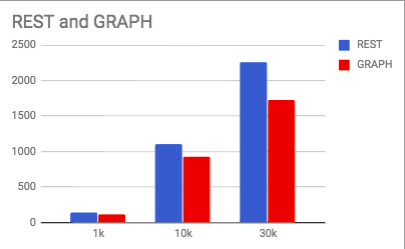
\includegraphics[width=0.8\textwidth]{figuras/Q1-result-request-time.png}
    \label{fig:q1-time}
    \caption{Comparação do tempo de resposta}
    \author{fonte: Autor}
\end{figure}

Com mil pallets cadastrados, a API REST teve como resultado um tempo de resposta de 147.3 ms, enquanto a API GraphQL respondeu a consulta em 115.63 ms, representando uma diferença de X por cento. Quando aumentamos o numero de pallets para 10 mil, a API REST respondeu as consultas em 1108.13 ms e a API GraphQL devolveu os resultados em 925.63 ms, uma diferença de Y por cento. Por último, as consultas com 30 mil pallets foram respondidas em 2261.1 ms na API REST e 1725.7 ms na API GraphQL, o que representa uma diferença de Z por cento.

\subsection{Tamanho da resposta}

Outro resultado esperado era que o tamanho da resposta da API GraphQL fosse menos do que o tamanho da resposta da API REST. Essa hipótese se confirmou como pode ser visto da figura \ref{fig:q1-size}.

\begin{figure}[htbp]
    \centering
    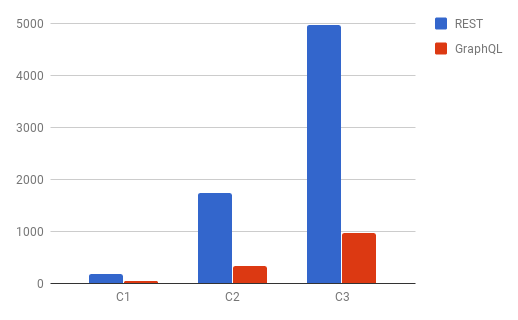
\includegraphics[width=0.8\textwidth]{figuras/Q1-size.png}
    \label{fig:q1-size}
    \caption{Comparação do tamanho de resposta}
    \author{fonte: Autor}
\end{figure}

A API REST respondeu as requisições da questão 1 com um tamanho de resposta de 174.04 Kb, 1740.17 Kb e 4980 Kb para mil pallets, 10 mil pallets e 30 mil pallets respectivamente. Da mesma maneira, a API GraphQL teve como resultado respostas com 31.68 Kb, 322.53Kb e 967.35Kb. 

\section{Questão 2}

Para as repostas da questão 2, as consultas foram mais complexas na API GraphQL, e mais numerosas na API REST. 

\subsection{Utilização da CPU}

\subsection{Consumo de memória}

\subsection{Tempo de resposta}

É possivel identificar com clareza, como mostra a figura \ref{fig:q2-time}, que a API REST leva um tempo consideravelmente maior para responder todas as requisições do que a consulta na API GraphQL.

\begin{figure}[htbp]
    \centering
    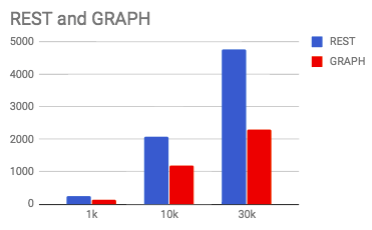
\includegraphics[width=0.8\textwidth]{figuras/Q2-result-request-time.png}
    \label{fig:q2-time}
    \caption{Comparação do tempo de resposta}
    \author{fonte: Autor}
\end{figure}

Com mil pallets cadastrados, a API REST teve como resultado um tempo de resposta de 254.56 ms, enquanto a API GraphQL respondeu a consulta em 148.5 ms, representando uma diferença de X por cento. Quando aumentamos o numero de pallets para 10 mil, a API REST respondeu as consultas em 2072.03 ms e a API GraphQL devolveu os resultados em 1201.3 ms, uma diferença de Y por cento. Por último, as consultas com 30 mil pallets foram respondidas em 4770.2 ms na API REST e 2291.1 ms na API GraphQL, o que representa uma diferença de Z por cento.

\subsection{Tamanho da resposta}

A API GraphQL também mostrou-se mais vantajosa em termos de tamho de resposta na Questão 2. A figura \ref{fig:q2-size} mostra a comparação entre os protótipos quando comparados o tamanho da resposta.

\begin{figure}[htbp]
    \centering
    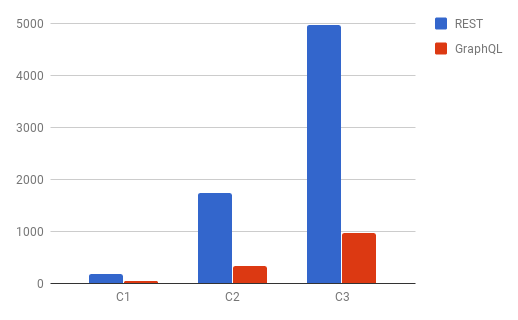
\includegraphics[width=0.8\textwidth]{figuras/Q1-size.png}
    \label{fig:q2-size}
    \caption{Comparação do tamanho de resposta}
    \author{fonte: Autor}
\end{figure}

A API REST respondeu as requisições da questão 1 com um tamanho de resposta de 259.53 Kb, 2522.17 Kb e 7221 Kb para mil pallets, 10 mil pallets e 30 mil pallets respectivamente. Da mesma maneira, a API GraphQL teve como resultado respostas com 101.73 Kb, 1005.23 Kb e 2850 Kb. 

    